\documentclass[11pt]{article}
\usepackage[T1]{fontenc}
\usepackage{lmodern,microtype,amsmath,amssymb,amsthm,mathtools}
\usepackage[margin=1in]{geometry}
\usepackage{graphicx,booktabs,array,xcolor,float}
\usepackage[colorlinks=true,linkcolor=blue!45!black,citecolor=blue!45!black,urlcolor=blue!45!black]{hyperref}
\usepackage{fancyhdr}
\pagestyle{fancy}\fancyhf{}\lhead{Small Integral Lifts of K3 Boundary Labels}\rhead{Shivam Gupta}\cfoot{\thepage}
\setlength{\headheight}{14pt}
\newtheorem{theorem}{Theorem}[section]
\newtheorem{proposition}[theorem]{Proposition}
\newtheorem{lemma}[theorem]{Lemma}
\newtheorem{corollary}[theorem]{Corollary}
\theoremstyle{remark}\newtheorem{remark}[theorem]{Remark}
\newcommand{\Z}{\mathbb Z}\newcommand{\Q}{\mathbb Q}\newcommand{\R}{\mathbb R}
\newcommand{\divis}{\operatorname{div}}\newcommand{\SL}{\operatorname{SL}}\newcommand{\htv}{\operatorname{ht}}
\title{Small Integral Lifts of K3 Boundary Labels:\\Exact Chart Heights and Saturated Quotient Certificates}
\author{Shivam Gupta\\\small Independent Researcher\\\small\href{mailto:shivam1720406@gmail.com}{shivam1720406@gmail.com}}
\date{17 October 2026}
\begin{document}
\maketitle
\begin{abstract}
The boundary of a polarized K3 period space is described by isotropic lattices, but computational use requires explicit integral representatives and saturated quotient bases. We give a deterministic construction for every isotropic discriminant label of the degree-$2d$ lattice. In the chart where one hyperbolic coordinate equals the divisibility $m$, the least coefficient height is exactly $m\min\{T\geq1:T(T+1)\geq (d/m^2)a^2\}$, with $a$ the centered residue of the label. Two explicit matrices in $\SL_2(\Z)$ transport a direct lift to this minimum. A Bezout calculation supplies a saturated basis of the orthogonal kernel and a certificate for the quotient $U\oplus2E_8(-1)\oplus\langle-2d/m^2\rangle$. Relative to the unrestricted minimum in the full K3 period lattice, the chart height is less than $\sqrt2$ times that minimum plus $m/2$; an explicit family makes the leading constant sharp. A separate example shows that the negative $E_8$ summands can improve height beyond the five-coordinate sublattice. Independent integer verification succeeds for 12,710 oriented labels with $d\leq4096$ and 500 large-integer cases. The contribution is an explicit height-controlled, certificate-producing realization of classical boundary arithmetic, rather than a new classification of K3 compactifications.
\end{abstract}
\noindent\textbf{Keywords:} K3 moduli; isotropic vectors; integral quadratic forms; coefficient height; exact computation; saturated lattices.\\
\textbf{Code and data:} \url{https://github.com/shi1720/k3-cusp-lifts}

\section{The computational question}
A zero-dimensional boundary component of an orthogonal modular variety is specified by an arithmetic orbit of rational isotropic lines. This description is intrinsic. Software, however, manipulates an integral primitive generator, a discriminant-group label, and an integral basis of its orthogonal quotient. Translating between those descriptions can introduce large coefficients or lose saturation. A vector of norm zero alone certifies neither the intended divisibility nor the integral quotient.

We consider the polarized K3 period lattice
\begin{equation}\label{eq:lattice}
 L_d=U_1\oplus U_2\oplus2E_8(-1)\oplus\Z g,\qquad g^2=-2d,\quad d>0.
\end{equation}
Each $U_i$ has basis $e_i,f_i$ with $(e_i,f_i)=1$ and $e_i^2=f_i^2=0$. Fix simple-root bases on the two negative $E_8$ summands. All coefficient heights in this paper refer to this fixed direct-sum basis; they are not invariants of an isometry class. Write
\[
 M_d=U_1\oplus U_2\oplus\Z g\subset L_d,
 \qquad v=(x_1,y_1,x_2,y_2,z).
\]
Then $v^2=2x_1y_1+2x_2y_2-2dz^2$. Our question is constructive: given the discriminant label of an isotropic primitive vector, how small a lift can be supplied with an independently checkable integral quotient?

The principal result is an exact optimum in a deliberately specified coordinate chart, not a global reduction algorithm. That optimum has a closed formula, an explicit stable isometry, and a saturated kernel basis. We also prove a comparison with the unrestricted full-lattice optimum and exhibit the obstruction to identifying the two. The software, called \emph{CuspLift}, returns all certificates as integers.

\begin{figure}[ht]
\centering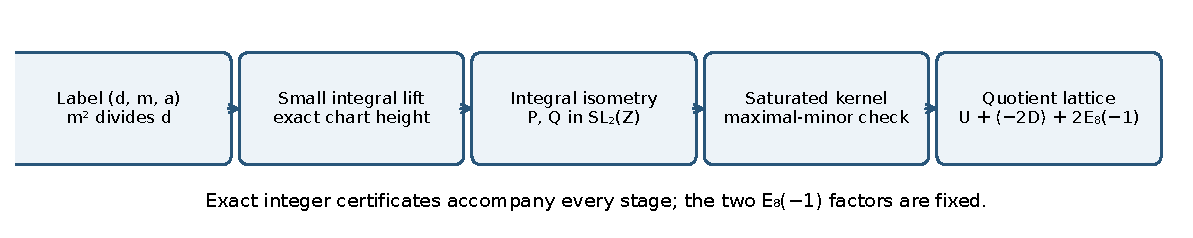
\includegraphics[width=\linewidth]{figures/workflow.pdf}
\caption{The certificate interface. The construction acts in $M_d$ and fixes both negative $E_8$ factors. Saturation is verified separately from the quotient Gram matrix.}\label{fig:workflow}
\end{figure}

\section{Classical context and scope of the contribution}
Scattone's analysis of polarized K3 boundary components already provides the underlying cusp classification \cite{scattone}. We use its rank-one setting, not its much richer classification of rank-two boundary components. The period-lattice description and the Eichler orbit criterion are reviewed by Gritsenko, Hulek, and Sankaran \cite{ghs}; the relevant statements in the cited arXiv version are Lemma~7.5 and Remarks~8.8--8.9. The geometric compactifications constructed by Alexeev and Engel \cite{ae} provide a broader setting in which explicit boundary data are useful. Our construction supplies no new toroidal fan, KSBA compactification, or degeneration of a surface.

Small-height zeros of quadratic forms have a substantial literature; Fukshansky surveys Cassels-type theorems and their extensions \cite{fuk}. Prescribed congruence conditions are also established territory \cite{bg}, as are conditions excluding finite-index sublattices \cite{fj}. Castel gives a factorization-free algorithm for finding isotropic vectors in general indefinite forms in dimension at least five \cite{castel}. Consequently, neither congruence-constrained isotropy nor avoidance of integer factorization is by itself a novelty claim here.

Our narrower contribution is the combination of an \emph{exact coordinate-chart height}, an explicit transport preserving the discriminant marking, and an embedded saturated quotient basis, with a full-lattice approximation bound and a sharpness family. The construction uses elementary determinant-preserving operations and Bezout's identity. The kernel isometry type and the orbit classification are classical consequences of the lattice theory. The formula and certificate interface are the technical results established directly below. The literature search did not identify this specific package of results in the sources examined; that is not a proof of absence from all prior work.

\subsection{Labels, signs, and the arithmetic group}
The discriminant group is $A_{L_d}\simeq\Z/(2d)$, with generator $g/(2d)$ and quadratic form
\begin{equation}\label{eq:disc}
 q(k)=-\frac{k^2}{2d}\pmod{2\Z}.
\end{equation}
For primitive $c$, let $m=\divis(c)$ be the positive generator of $(c,L_d)\subset\Z$. The class $c/m+L_d$ has order $m$. An element of order $m$ has the form $k=(2d/m)a$, with $a\in(\Z/m)^\times$. Isotropy of this class is equivalent to $m^2\mid d$, since $q(k)=-2da^2/m^2$ and $\gcd(a,m)=1$.

Thus an \emph{oriented label} is a pair
\begin{equation}\label{eq:label}
 (m,a),\qquad m^2\mid d,\quad a\in(\Z/m)^\times.
\end{equation}
For $m=1$, the residue is $a=0$. We always choose the centered integer representative $-m/2<a\leq m/2$. In the two-hyperbolic-plane setting, the classical Eichler criterion identifies the primitive-vector orbit under the stable special orthogonal group by norm and discriminant class. We use that criterion only to interpret the supplied lifts as representatives of all labels.

For completeness, write $d=s\ell^2$ with $s$ squarefree. The square divisors $m^2\mid d$ are exactly $m\mid\ell$, so the number of oriented labels is $\sum_{m\mid\ell}\varphi(m)=\ell$. Sign reversal fixes only the order-one label and, when $2\mid\ell$, the order-two label. Thus the number of sign classes is $\lfloor\ell/2\rfloor+1$. These are elementary consequences of the classical label description.

Lines have no preferred sign: $c$ and $-c$ generate the same line. The corresponding sign quotient identifies $a$ with $-a$. No further quotient by the full automorphism group of $A_{L_d}$ is taken here. Our atlas counts oriented labels, not distinct zero-dimensional cusps. This distinction matters when comparing its sizes with boundary tables.

\section{An exact chart minimum}
Fix a label, put $D=d/m^2$, and define $S=Da^2$. Consider the following chart of lifts in $M_d$:
\begin{equation}\label{eq:chart}
 \mathcal C_{d,m,a}=\{(mx,my,m,mw,z):x,y,w,z\in\Z,\ z\equiv a\pmod m,\ v^2=0\}.
\end{equation}
Every vector in this chart has divisibility exactly $m$: one of its hyperbolic coordinates is $m$, all hyperbolic coordinates are multiples of $m$, and $m\mid2dz$. It is primitive because $\gcd(z,m)=1$. Its label is the one specified in \eqref{eq:label}. These statements include the case $m=1$.

\begin{theorem}[Chart height]\label{thm:chart}
Let
\begin{equation}\label{eq:T}
 T=T(S)=\min\{t\in\Z_{\geq1}:t(t+1)\geq S\}.
\end{equation}
The minimum coefficient height on $\mathcal C_{d,m,a}$ is $mT$. Define
\begin{equation}\label{eq:construction}
 y=\min\{T,\lfloor S/T\rfloor\},\qquad w=S-Ty.
\end{equation}
A minimizing vector is
\begin{equation}\label{eq:c}
 c=(mT,my,m,mw,a).
\end{equation}
The construction uses one integer square root, integer division, and a bounded number of arithmetic operations after the label has been supplied.
\end{theorem}
\begin{proof}
For $v$ as in \eqref{eq:chart}, isotropy is $xy+w=Dz^2$. Since $a$ is centered, $|z|\geq|a|$. If the height of $v$ is less than $mt$, its three normalized coordinates $x,y,w$ have absolute value at most $t-1$, so
\[
 S\leq Dz^2=xy+w\leq(t-1)^2+(t-1).
\]
This excludes every height less than $mT$: for $T>1$, minimality in \eqref{eq:T} gives $(T-1)T<S$, and for $T=1$ the coordinate $m$ itself is a lower bound.

For existence, if $S\leq T^2$, integer division in \eqref{eq:construction} gives $0\leq y\leq T$ and $0\leq w<T$. If $T^2<S\leq T^2+T$, it gives $y=T$ and $0<w\leq T$. In both cases $Ty+w=S$, hence \eqref{eq:c} is isotropic. Its largest hyperbolic coefficient is $mT$. Also $|a|\leq m/2$ when $m>1$, and $a=0$ for $m=1$. Thus its height is exactly $mT$.
\end{proof}

The positive-real root of $t(t+1)=S$ gives
\[
 T=\max\left\{1,\left\lceil\frac{\sqrt{1+4S}-1}{2}\right\rceil\right\}.
\]
The implementation does not use a floating-point square root. It computes $r=\lfloor\sqrt{1+4S}\rfloor$, initializes $t=\max\{1,\lfloor(r-1)/2\rfloor\}$, and increments once if $t(t+1)<S$.

\subsection{A direct lift and its explicit transport}
The simple direct lift
\begin{equation}\label{eq:seed}
 c_0=(m,mS,0,0,a)
\end{equation}
is already primitive, isotropic, and correctly labelled. Its height is $m\max\{1,S\}$. Represent the four hyperbolic coordinates by
\[
 X(v)=\begin{pmatrix}x_1&x_2\\-y_2&y_1\end{pmatrix},\qquad \det X(v)=x_1y_1+x_2y_2.
\]
For $P,Q\in\SL_2(\Z)$, the map $X\mapsto PXQ$ preserves this determinant, hence the quadratic form on $2U$. With $y,w$ as above, take
\begin{equation}\label{eq:PQ}
 P=\begin{pmatrix}1&0\\y&1\end{pmatrix},\qquad
 Q=\begin{pmatrix}T&1\\-1&0\end{pmatrix}.
\end{equation}
Direct multiplication yields
\[
 P\begin{pmatrix}m&0\\0&mS\end{pmatrix}Q
 =\begin{pmatrix}mT&m\\-mw&my\end{pmatrix}=X(c).
\]
Extend this map, denoted $\Phi$, by the identity on $g$ and both negative $E_8$ factors. It is an integral isometry, acts trivially on the discriminant group, and belongs to the identity component over $\R$: both $\SL_2(\R)$ factors are connected, and the displayed action is continuous. In particular, it preserves the chosen period-domain component. This is a constructive equivalence certificate; testing equality of norms would be insufficient.

\section{An embedded, saturated quotient certificate}
An isometry type of a rational quotient does not by itself identify an integral quotient. We give a basis of the complete integral orthogonal kernel before passing to $c^\perp/\Z c$.

\begin{theorem}[Kernel and quotient]\label{thm:quotient}
Choose integers $u,v$ satisfying $mv-au=1$, and set
\begin{align*}
 b_1&=(1,-Da^2,0,0,0),& b_2&=(0,2mDa,0,0,1),\\
 b&=u b_1+v b_2,& E&=(0,0,1,0,0),\quad F=(0,0,0,1,0).
\end{align*}
Then $c_0,b,E,F$ form a $\Z$-basis of $c_0^\perp\cap M_d$. Their transforms $c,\Phi(b),\Phi(E),\Phi(F)$ form a saturated basis of $c^\perp\cap M_d$, with Gram matrix
\begin{equation}\label{eq:kernelgram}
 \begin{pmatrix}0&0&0&0\\0&-2D&0&0\\0&0&0&1\\0&0&1&0\end{pmatrix}.
\end{equation}
Consequently,
\begin{equation}\label{eq:quotient}
 c^\perp_{L_d}/\Z c\simeq U\oplus2E_8(-1)\oplus\langle-2D\rangle.
\end{equation}
\end{theorem}
\begin{proof}
In $U_1\oplus\Z g$, orthogonality to $c_0$ is the integer equation
\[
 y_1=2mDa z-Da^2x_1.
\]
Its full solution lattice is freely generated by $b_1,b_2$. Since $c_0=mb_1+ab_2$ and
\[
 \det\begin{pmatrix}m&u\\a&v\end{pmatrix}=1,
\]
the pair $c_0,b$ is another integral basis, not merely a finite-index sublattice. The second hyperbolic plane is orthogonal to these vectors. A calculation gives $b^2=-2D(au-mv)^2=-2D$, while $(b,c_0)=0$. This proves the kernel Gram matrix for the seed. The integral automorphism $\Phi$ transports the basis and preserves saturation. Finally, add the unchanged $2E_8(-1)$ basis and quotient out its primitive radical generator $c$.
\end{proof}

\subsection{Independent saturation verification}
The verifier uses no knowledge of how the Bezout basis was constructed. Let $B$ be the $5\times4$ matrix of the returned kernel vectors, and $G$ the Gram matrix of $M_d$. The primitive annihilator of $c^\perp\cap M_d$ is
\[
 n=Gc/m\in\Z^5,\qquad \gcd(n_1,\ldots,n_5)=1.
\]
Define $h_i=(-1)^{i-1}\det B_{\widehat i}$, where row $i$ is deleted. We require
\begin{equation}\label{eq:cofactor}
 h=n\quad\text{or}\quad h=-n.
\end{equation}
The vector $h$ annihilates the columns of $B$. Its coordinate gcd is the index of their span in the saturated rank-four lattice in the same rational subspace. Thus \eqref{eq:cofactor} certifies both the correct kernel and index one. This check detects a finite-index error even when the rational orthogonal space is correct. The verifier additionally checks the claimed Gram matrix, the primitive vector, its norm, divisibility, discriminant label, and the full $5\times5$ isometry induced by $P,Q$.

For normalized input labels, all returned integers have $O(\log d)$ bits. The number of integer operations outside extended Euclid and integer square root is bounded independently of $d$. Verification uses fixed-size determinants and pairings, so it too has polynomial bit complexity. This statement concerns a \emph{supplied label}. Enumerating square divisors by scanning to $\sqrt d$, as our atlas script does, is not polynomial in the bit length of $d$.

\section{Comparison with unrestricted representatives}
Let $H_{\mathrm{all}}(d,m,a)$ be the least coefficient height among all primitive isotropic vectors of $L_d$ with the specified label. Let $H_5$ be the analogous minimum restricted to $M_d$. The chart height is $H_{\mathrm{chart}}=mT$. These satisfy
\[
 H_{\mathrm{all}}\leq H_5\leq H_{\mathrm{chart}},
\]
but either inequality can be strict.

\begin{theorem}[Full-lattice bound and sharp leading constant]\label{thm:comparison}
For every nontrivial label ($m>1$),
\begin{equation}\label{eq:bound}
 H_{\mathrm{all}}\geq m\left\lceil\sqrt{S/2}\right\rceil,
 \qquad H_{\mathrm{chart}}<\sqrt2\,H_{\mathrm{all}}+\frac m2.
\end{equation}
No constant smaller than $\sqrt2$ can replace the leading constant in a uniform inequality of the second form with an additive term $O(m)$.
\end{theorem}
\begin{proof}
Write an unrestricted vector as $c'=(x_1,y_1,x_2,y_2,z,\eta)$, with $\eta\in2E_8(-1)$. Divisibility $m$ forces all four hyperbolic coordinates to be multiples of $m$. Its discriminant class forces $z\equiv a\pmod m$, so $|z|\geq|a|$. As $\eta^2\leq0$, isotropy implies
\[
 x_1y_1+x_2y_2=dz^2-\eta^2/2\geq da^2=m^2S.
\]
If the largest normalized hyperbolic coefficient is $K$, the left side is at most $2m^2K^2$. Therefore $K\geq\lceil\sqrt{S/2}\rceil$ and $H_{\mathrm{all}}\geq mK$. For positive integer $S$, minimality and integrality give $S\geq T^2-T+1>(T-1/2)^2$, hence $T<\sqrt S+1/2$. Combining with $m\sqrt S\leq\sqrt2 H_{\mathrm{all}}$ proves the second inequality.

For sharpness, let $m=3$, $a=1$, $D=k(2k-1)$, and $d=9D$, for integers $k\geq2$. The vector
\begin{equation}\label{eq:sharp}
 (3k,3k,3(k-1),3k,1,0,\ldots,0)
\end{equation}
is primitive, has divisibility three, and is isotropic, of height $3k$. Since $2(k-1)^2<k(2k-1)\leq2k^2$, the lower bound in \eqref{eq:bound} is $3k$. Thus $H_{\mathrm{all}}=H_5=3k$, whereas $H_{\mathrm{chart}}=3T(k(2k-1))$ and $T(k(2k-1))/k\to\sqrt2$. An additive $O(m)$ term cannot change this limit as $k\to\infty$.
\end{proof}

\subsection{Two distinct failures of global optimality}
For $d=819$, $m=3$, $a=1$, we have $S=91$, $T=10$, $y=9$, $w=1$. The chart gives
\[
 c=(30,27,3,3,1),\qquad H_{\mathrm{chart}}=30.
\]
The vector $(21,21,18,21,1)$ has the same label and height 21. Theorem~\ref{thm:comparison} gives the lower bound $3\lceil\sqrt{91/2}\rceil=21$, so $H_5=H_{\mathrm{all}}=21$. In particular $30/21=10/7>\sqrt2$: deleting the additive term from \eqref{eq:bound} would be false.

The negative-definite factors create a different effect. Let $d=63$, $m=3$, $a=1$; now $S=7$ and the chart height is 9. In the five-coordinate sublattice, height at most 6 would require $xy+uw=7$ with all four normalized coordinates bounded by two. Products of integers in $[-2,2]$ belong to $\{-4,-2,-1,0,1,2,4\}$; no two sum to seven. Hence $H_5=9$.

Let $\alpha$ be a simple root of one $E_8(-1)$ factor, so $\alpha^2=-2$. The full-lattice vector
\begin{equation}\label{eq:E8example}
 c'=(6,6,6,6,1)+3\alpha
\end{equation}
has norm $144-126-18=0$. It is primitive, has divisibility three (a neighboring simple root pairs with $3\alpha$ to give $3$), and has the same label. Its height is six. The full-lattice lower bound is $3\lceil\sqrt{7/2}\rceil=6$, so $H_{\mathrm{all}}=6<H_5=9$. Thus a five-coordinate search must not be reported as full-lattice height optimization.

\section{Reproducible computational study}
The experiments audit the proved construction and characterize coefficient sizes. They do not estimate a success probability for a conjecture. All finite datasets are deterministic except the explicitly seeded large-integer and timing inputs. The core constructor and verifier use the Python standard library; plots additionally use NumPy and Matplotlib.

\subsection{Exhaustive labels and independent checks}
For every $1\leq d\leq4096$, we enumerate the labels in \eqref{eq:label} and compare their discriminant residues with a separate direct scan of all $0\leq k<2d$ satisfying $k^2\equiv0\pmod{4d}$. Equality of these sets checks completeness of label enumeration independently of the constructor. Each label receives the full certificate checks described above. Both signs are retained.

The resulting 12,710 certificates all verify. Of these, 8,614 have $m>1$; 8,489 strictly improve the direct seed height, and 125 tie. The median seed-to-chart height ratio on nontrivial labels is $12.1667$ and the maximum is $32$. All trivial labels tie at height one. These ratios compare against the explicit seed \eqref{eq:seed}, not against a general-purpose lattice reduction package.

\begin{table}[ht]
\centering
\caption{Selected degrees. Oriented labels retain sign; the next column quotients by sign. Heights are maxima over the oriented labels at that degree.}\label{tab:degrees}
\begin{tabular}{rrrrr}\toprule
$d$ & Oriented labels & Sign classes & Direct seed height & Chart height\\\midrule
1&1&1&1&1\\
4&2&2&2&2\\
9&3&2&3&3\\
36&6&4&18&6\\
100&10&6&90&30\\
900&30&16&5,070&390\\
3,600&60&31&50,460&1,740\\
4,096&64&33&61,504&1,984\\\bottomrule
\end{tabular}
\end{table}

\begin{figure}[ht]
\centering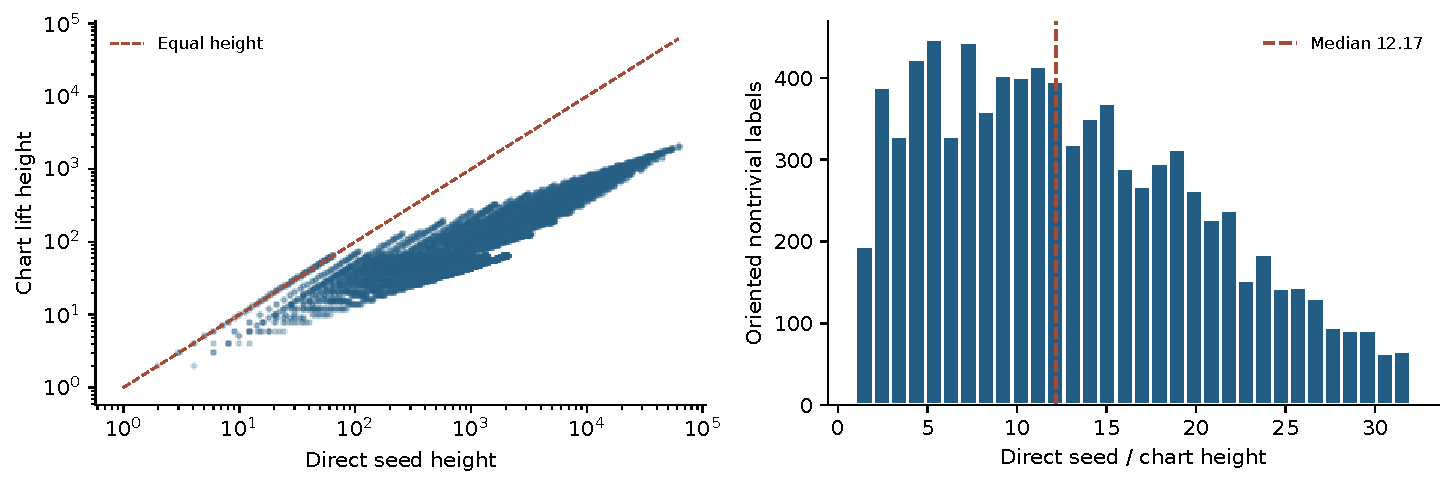
\includegraphics[width=\linewidth]{figures/height_atlas.pdf}
\caption{The 8,614 nontrivial oriented labels with $d\leq4096$. Left: coefficient heights against the simple direct lift; the dashed diagonal denotes a tie. Right: the distribution of height reduction ratios. Repeated or symmetric labels remain in the dataset; these are finite atlas statistics, not independent samples.}\label{fig:atlas}
\end{figure}

A second calculation minimizes $\max\{1,|x|,|y|,|S-xy|\}$ by direct enumeration for all $0\leq S\leq1024$. The 1,025 minima agree with $T(S)$. This check derives the residual coordinate from the norm equation and does not call the chart constructor.

For each $1\leq S\leq1024$, we also set $(d,m,a)=(9S,3,1)$ and compute the exact five-coordinate minimum \emph{at the fixed centered value $z=1$}. At a candidate normalized height $K$, a product table lists all $(x,y)\in[-K,K]^2$ by $xy$. We match products summing to $S$, and test $\gcd(x,y,u,w,6S)=1$ for divisibility three. Searching increasing $K$ certifies the first feasible height, and the chart provides the stopping bound. The largest observed chart-to-fixed-$z$ ratio is $10/7$. We intentionally report this as a fixed-$z$ study, not an exhaustive search through the full rank-21 lattice.

\begin{figure}[ht]
\centering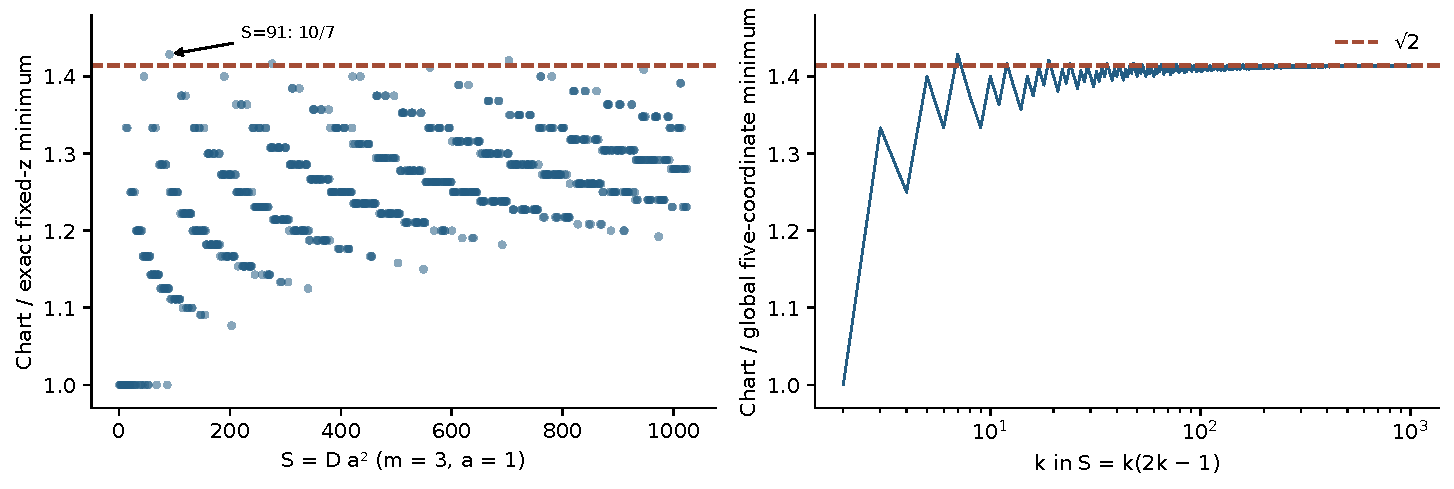
\includegraphics[width=\linewidth]{figures/optimality_gap.pdf}
\caption{Height comparisons with distinct domains. Left: exact fixed-$z$ five-coordinate enumeration for $S=1,\ldots,1024$. Right: the explicit family \eqref{eq:sharp}, whose unrestricted full-lattice minimum is proved, for $k=2,\ldots,1000$. The dashed line is $\sqrt2$; finite ratios can exceed it, consistently with the additive term in Theorem~\ref{thm:comparison}.}\label{fig:gap}
\end{figure}

\subsection{Large integers, failure detection, and cost}
Using Python's pseudorandom generator with seed 6052026, we generate 500 cases with $2\leq m<250$, a uniformly sampled unit residue obtained by rejection, and $D=1+\operatorname{getrandbits}(256)$. Every certificate verifies. Five deliberate mutations are rejected: a changed hyperbolic coordinate, a changed $g$ coordinate, a doubled kernel basis vector, an altered isometry matrix, and an incorrect divisibility parameter. These are targeted tests of meaningful failure modes, not a claim of adversarial completeness. A separate 21-coordinate script verifies \eqref{eq:E8example} using an explicit negative $E_8$ Cartan matrix.

\begin{table}[ht]
\centering
\caption{Descriptive per-case median times in microseconds, 40 inputs per row, $m=7$, $a=3$. Construction includes the quotient basis; verification includes rational determinant calculations.}\label{tab:timing}
\begin{tabular}{rrr}\toprule
Bit length of $D$ & Construction & Independent verification\\\midrule
16&16.67&381.21\\
64&17.81&405.77\\
128&18.08&412.90\\
256&18.33&418.69\\
512&19.65&457.40\\
1,024&21.85&525.96\\\bottomrule
\end{tabular}
\end{table}

The recorded environment is CPython 3.9.6 on an ARM64 macOS host. Measurements use \texttt{perf\_counter\_ns} in one process, with no machine isolation; they are descriptive, not a cross-system performance comparison. The timings show that the reference certificate checks cost more than the construction, which is expected for a verifier using exact rational elimination. The exhaustive atlas construction, direct residue scan, and certificate verification together took 6.11 seconds in the recorded run. Broader claims about acceleration of moduli computations would require a downstream workload and a comparison against established implementations, which we have not performed.

\section{Use in boundary computation and remaining questions}
The immediate application is a reusable arithmetic interface for polarized K3 boundary data: given $(d,m,a)$, return a representative, an explicit stable isometry, an embedded saturated kernel basis, and the quotient Gram matrix. This can support initialization of local cusp calculations, regression tests for computer-algebra implementations, and interchange of boundary data between independently implemented systems. Because the certificates contain only integers, downstream code can check them without trusting the constructor or repeating a search. The construction exploits the fixed split form of $L_d$; a general Gram matrix first needs a certified identification with that form.

There are practical limits. Smaller coordinates of $c$ need not make the entire quotient basis smaller: Bezout coefficients and the transported basis can grow. No improvement in end-to-end running time for compactification algorithms is established. The method does not compute rank-two boundary incidence, degenerations, or fans, and it provides no classification of geometric central fibers. Its coefficient height is basis-dependent. The global comparison theorem bounds a search domain but does not solve the unrestricted optimization problem.

For scientific software, the useful deliverable is a verified primitive that can be embedded in a larger arithmetic geometry pipeline. A commercial implementation could supply supported exact-arithmetic tooling or validation infrastructure, but this study contains no customer evidence, market-size estimate, or patentability assessment. Such claims would not follow from a coefficient-height theorem.

The examples suggest two precise next questions. First, can bounded vectors in the negative $E_8$ factors be used to characterize the exact full-lattice minimum, closing the gaps in the two-product table? Second, can representative height and quotient-basis height be optimized jointly while retaining a short integral equivalence certificate? The $D=7$ example shows why the first question requires the full lattice, while the explicit transport makes the second testable. Both extend the present certificate interface without conflating it with the established geometry of compactifications.

\appendix
\section{Executable contract and reproduction}
The repository contains \texttt{src/cusp\_lifts.py}, the independent \texttt{src/verify.py}, the full study script, raw certificate files, CSV tables, and figure sources. From the repository root:
\begin{verbatim}
python3 tests/run_study.py
python3 tests/full_lattice_example.py
python3 src/verify.py results/certificates.jsonl
python3 paper/make_figures.py
tectonic paper/manuscript/main.tex
\end{verbatim}
The first script regenerates all mathematical study data and descriptive timing values; the last command produces the PDF beside the TeX source. The committed timing table records the original run and may differ on another host. The integer verifier rejects invalid certificates even when Python optimization is enabled; its checks do not rely on removable \texttt{assert} statements. The study harness itself should be run without \texttt{-O}.

All integral bases are recorded as \emph{lists of column vectors}; consumers must transpose that list when forming a conventional basis matrix. The verifier explicitly checks the signed maximal minors, preventing a row/column convention error from silently changing the lattice.

\begin{thebibliography}{9}
\small\raggedright\setlength{\itemsep}{0pt}
\bibitem{scattone} F. Scattone. \emph{On the compactification of moduli spaces for algebraic K3 surfaces}. Memoirs of the American Mathematical Society 70, no. 374, 1987. \href{https://doi.org/10.1090/memo/0374}{doi:10.1090/memo/0374}.
\bibitem{ghs} V. Gritsenko, K. Hulek, and G. K. Sankaran. Moduli of K3 surfaces and irreducible symplectic manifolds. In \emph{Handbook of Moduli}, vol. I, Advanced Lectures in Mathematics 24, pp. 459--526. International Press, 2013. \href{https://arxiv.org/abs/1012.4155}{arXiv:1012.4155v2}.
\bibitem{ae} V. Alexeev and P. Engel. \emph{Compact moduli of K3 surfaces}. \href{https://arxiv.org/abs/2101.12186}{arXiv:2101.12186v3}, 2023.
\bibitem{fuk} L. Fukshansky. Heights and quadratic forms: Cassels' theorem and its generalizations. \emph{Contemporary Mathematics} 587 (2013), 77--94. \href{https://arxiv.org/abs/1204.1938}{arXiv:1204.1938}.
\bibitem{bg} P. Bandi and A. Ghosh. \emph{Small solutions of quadratic forms with congruence conditions}. \href{https://arxiv.org/abs/2008.08568}{arXiv:2008.08568v2}, 2020.
\bibitem{fj} L. Fukshansky and S. Jeong. \emph{Integral zeros of quadratic polynomials avoiding sublattices}. \href{https://arxiv.org/abs/2409.10867}{arXiv:2409.10867v2}, 2024.
\bibitem{castel} P. Castel. Solving quadratic equations in dimension 5 or more without factoring. \emph{The Open Book Series} 1 (2013), 213--234. \href{https://doi.org/10.2140/obs.2013.1.213}{doi:10.2140/obs.2013.1.213}.
\end{thebibliography}
\end{document}
